\documentclass[12pt,a4paper,oneside]{book}
\usepackage[utf8]{inputenc}
\usepackage[spanish,es-tabla]{babel}
\usepackage[left=3.5cm,right=2.5cm,top=2.5cm,bottom=2.5cm]{geometry}
\usepackage{amsmath,amssymb,amsfonts}
\usepackage{graphicx}
\usepackage{booktabs}
\usepackage{array}
\usepackage{setspace}
\usepackage{fancyhdr}
\usepackage{titlesec}
\usepackage{hyperref}
\usepackage{listings}
\usepackage{color}
\usepackage{microtype}
\usepackage{caption}
\usepackage{subcaption}

\onehalfspacing
\setlength{\parskip}{6pt}
\setlength{\parindent}{0pt}

\hypersetup{
    colorlinks=true,
    linkcolor=black,
    citecolor=black,
    urlcolor=blue,
    pdftitle={Sistema Agéntico para Diseño de Perforación y Voladura - UNI FIGMM},
    pdfauthor={Bachiller en Ingeniería de Minas},
    pdfsubject={Tesis de Titulación Profesional}
}

% Formato de encabezados
\pagestyle{fancy}
\fancyhf{}
\fancyhead[R]{\small\nouppercase{\leftmark}}
\fancyfoot[C]{\thepage}
\renewcommand{\headrulewidth}{0.5pt}

\begin{document}

% -------------------------------------------------------------
% PORTADA OFICIAL UNI FIGMM
% -------------------------------------------------------------
\begin{titlepage}
\begin{center}
    {\fontsize{16}{20}\selectfont \textbf{UNIVERSIDAD NACIONAL DE INGENIERÍA}}\\[0.3cm]
    {\fontsize{14}{18}\selectfont \textbf{FACULTAD DE INGENIERÍA GEOLÓGICA, MINERA Y METALÚRGICA}}\\[0.2cm]
    {\fontsize{12}{16}\selectfont \textbf{ESCUELA PROFESIONAL DE INGENIERÍA DE MINAS}}\\[1.0cm]
    
    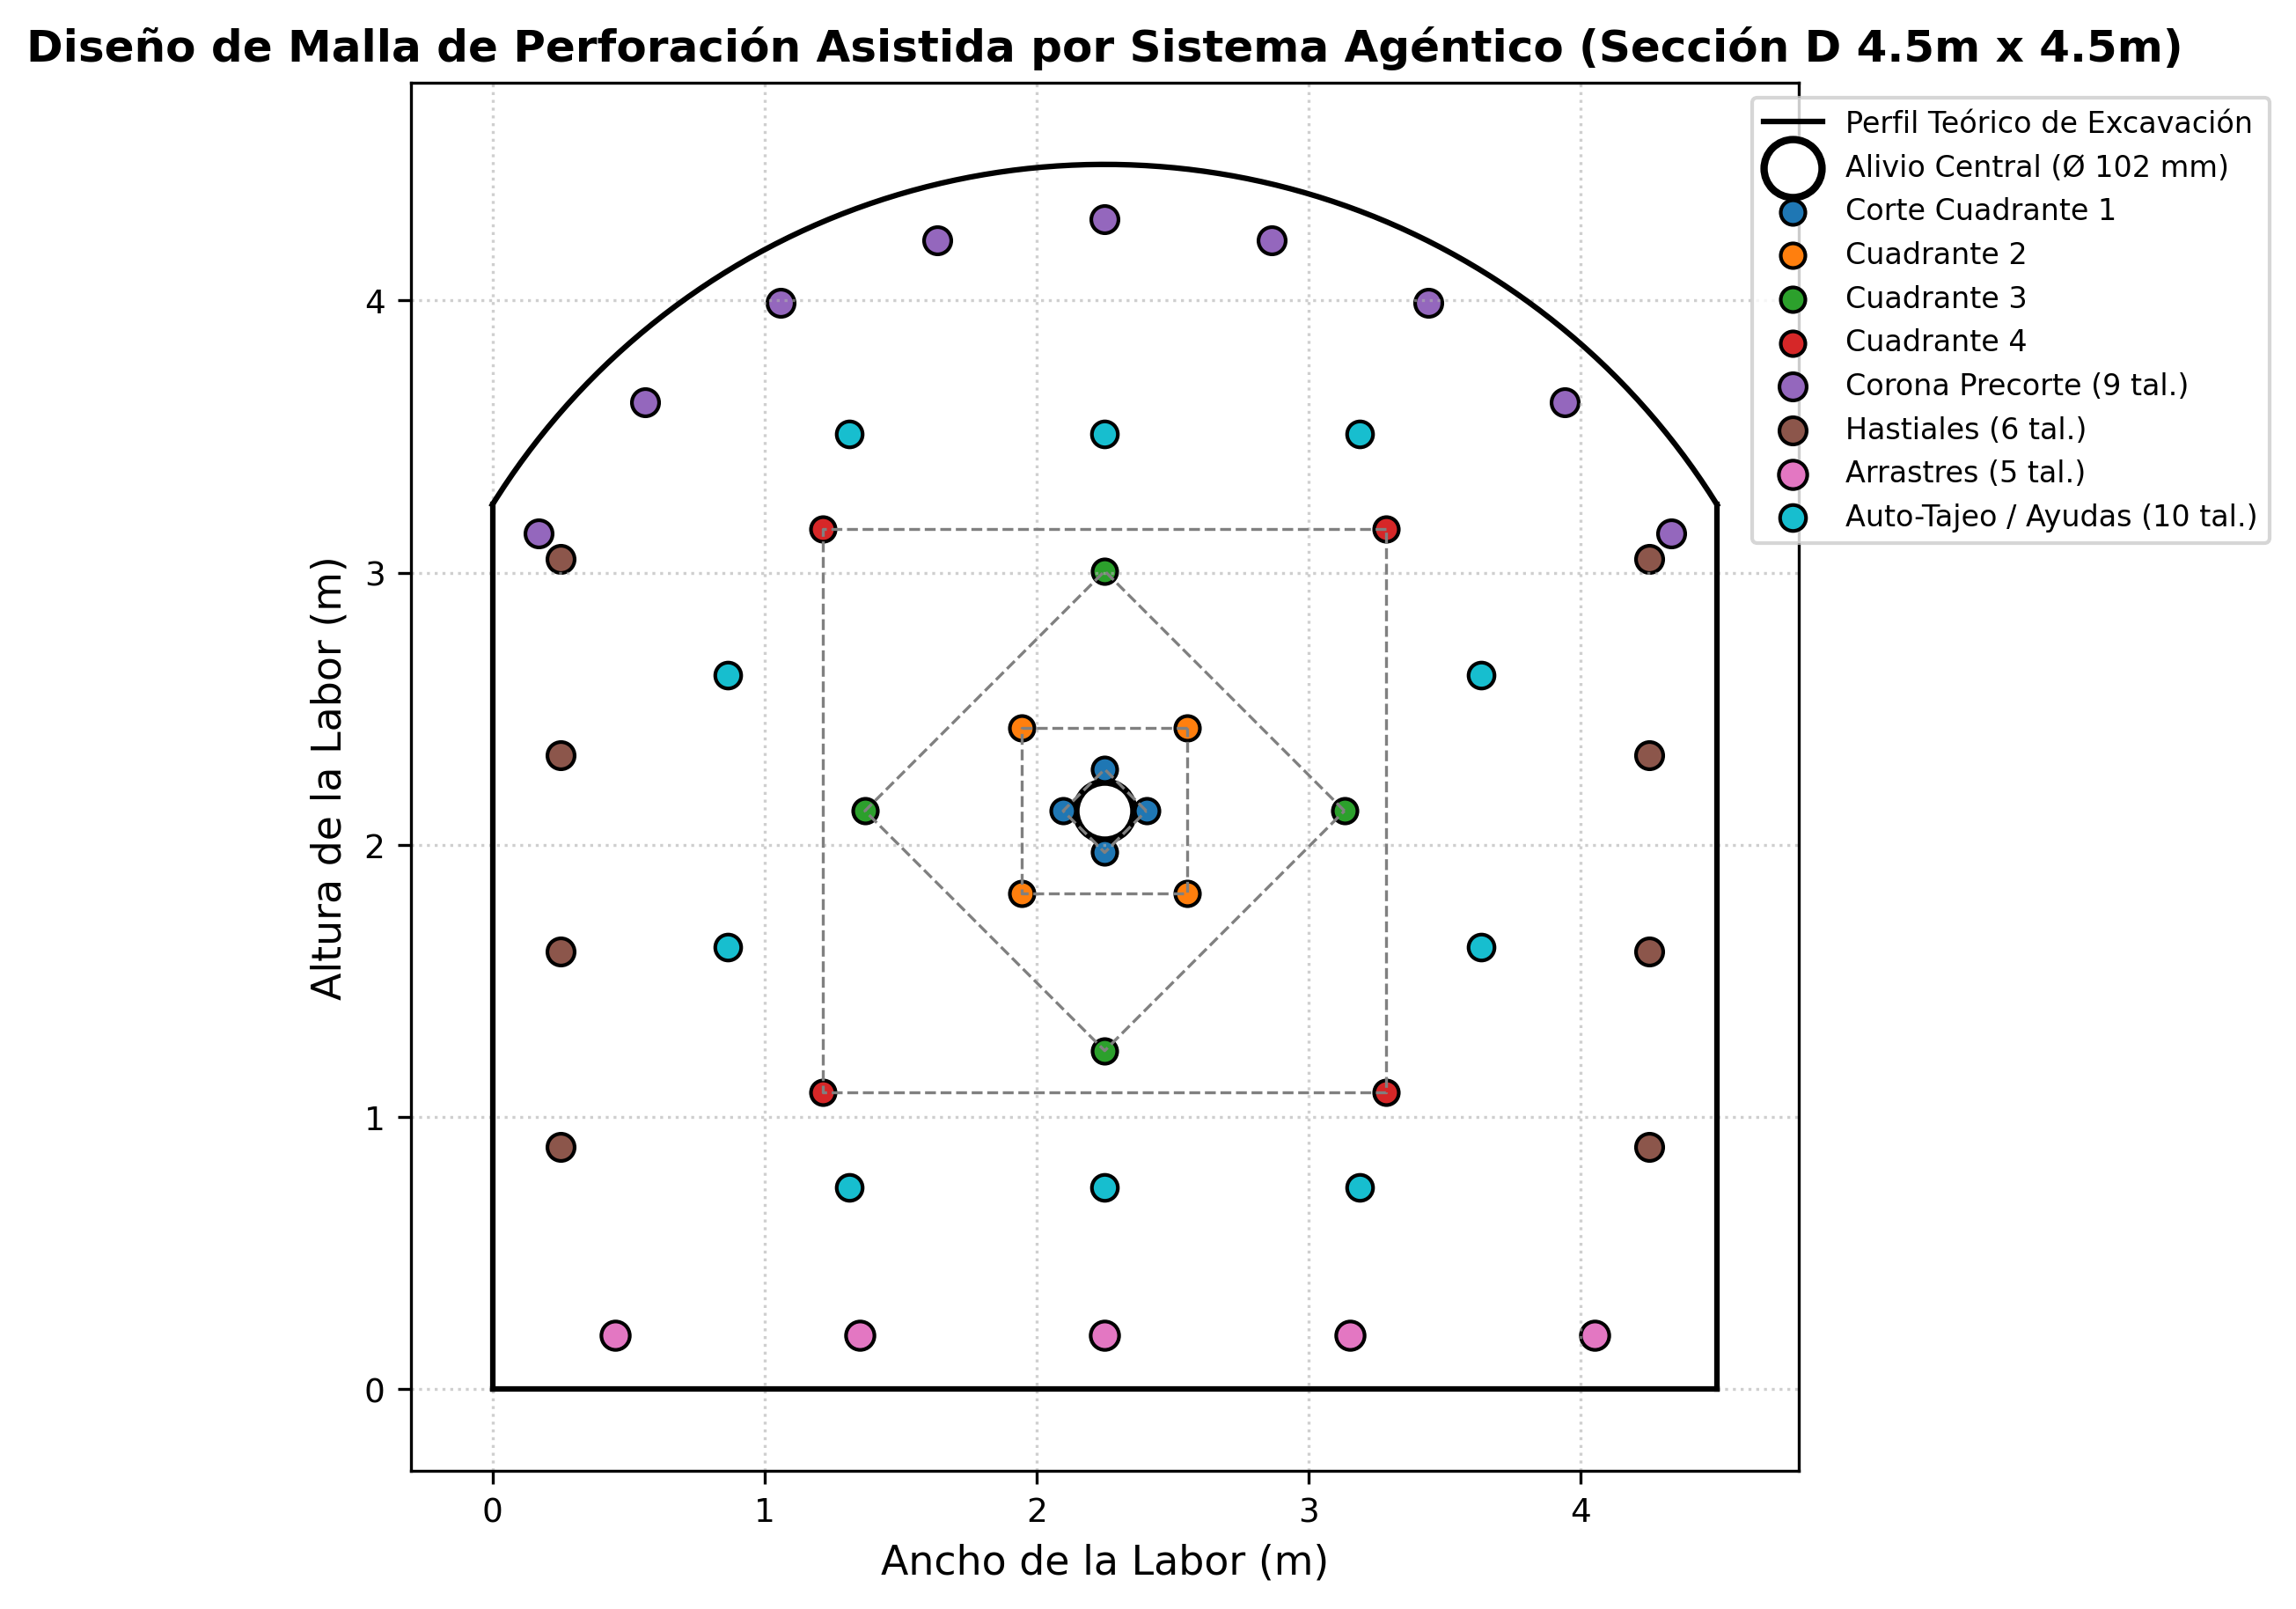
\includegraphics[width=3.5cm]{figures/figura_01_malla_perforacion.png}\\[1.0cm]
    
    {\fontsize{14}{18}\selectfont \textbf{TESIS}}\\[0.5cm]
    
    {\fontsize{14}{18}\selectfont \textbf{SISTEMA AGÉNTICO BASADO EN INTELIGENCIA ARTIFICIAL PARA EL DISEÑO ASISTIDO DE PERFORACIÓN Y VOLADURA ORIENTADO AL CONTROL DE LA SOBREROTURA EN LABORES SUBTERRÁNEAS DE LA U.E.A. LINCUNA, 2026}}\\[1.2cm]
    
    {\fontsize{12}{15}\selectfont PARA OPTAR EL TÍTULO PROFESIONAL DE:}\\[0.2cm]
    {\fontsize{13}{16}\selectfont \textbf{INGENIERO DE MINAS}}\\[1.2cm]
    
    {\fontsize{12}{15}\selectfont PRESENTADO POR:}\\[0.2cm]
    {\fontsize{12}{15}\selectfont \textbf{BACHILLER EN CIENCIAS CON MENCIÓN EN INGENIERÍA DE MINAS}}\\[0.8cm]
    
    {\fontsize{12}{15}\selectfont ASESOR:}\\[0.2cm]
    {\fontsize{12}{15}\selectfont \textbf{DR. ING. ASESOR DE TESIS (UNI FIGMM)}}\\[1.2cm]
    
    {\fontsize{12}{15}\selectfont \textbf{LIMA -- PERÚ}}\\[0.2cm]
    {\fontsize{12}{15}\selectfont \textbf{2026}}
\end{center}
\end{titlepage}

\frontmatter

% -------------------------------------------------------------
% DEDICATORIA Y AGRADECIMIENTOS
% -------------------------------------------------------------
\chapter*{Dedicatoria}
\addcontentsline{toc}{chapter}{Dedicatoria}
\textit{A mis padres, por su apoyo incondicional y sus sacrificios a lo largo de toda mi formación universitaria. A la memoria de los maestros de la Universidad Nacional de Ingeniería, por inculcar el rigor científico y el compromiso inquebrantable con el desarrollo del sector minero peruano.}

\chapter*{Agradecimientos}
\addcontentsline{toc}{chapter}{Agradecimientos}
A la \textbf{Universidad Nacional de Ingeniería} y a la \textbf{Facultad de Ingeniería Geológica, Minera y Metalúrgica (FIGMM)}, por brindarme una formación técnica de excelencia y valores éticos profesionales.

A la \textbf{Compañía Minera Lincuna S.A.}, por la apertura técnica, la confianza brindada en interior mina y la facilitación de las bases de datos operacionales y frentes de avance para la ejecución de las pruebas experimentales.

A mi asesor de tesis, por su orientación metodológica, rigurosidad académica y valiosos aportes en el campo de la geomecánica y la computación científica aplicada.

% -------------------------------------------------------------
% RESUMEN Y ABSTRACT
% -------------------------------------------------------------
\chapter*{Resumen}
\addcontentsline{toc}{chapter}{Resumen}
La presente investigación aborda el problema crítico de la sobre-excavación o sobrerotura (\textit{overbreak}) en las labores subterráneas de desarrollo horizontal (cruceros y galerías de nivel en sección D de $4.50\text{ m} \times 4.50\text{ m}$) de la U.E.A. Lincuna, Áncash. Históricamente, la operación presentaba un índice medio de sobrerotura del $34.36\%$ debido al uso de mallas de perforación empíricas, sobrecarga de explosivos y ausencia de voladura controlada desacoplada en el contorno, generando sobrecostos de sostenimiento con concreto lanzado (\textit{shotcrete}) de $\$7,639.50\text{ USD}$ por disparo y graves riesgos de caída de rocas. 

Para solucionar esta problemática, se desarrolló e implementó un **Sistema Agéntico Autónomo Multi-Rol basado en Inteligencia Artificial y Reglas Físicas Determinísticas**, integrando el modelo matemático de Holmberg-Persson para 5 secciones de confinamiento y un algoritmo heurístico de auto-tajeo espacial ($S/B = 1.25, f = 1.45$). La gobernanza del sistema verifica rigurosamente que la presión efectiva en pared de taladro ($P_{te} = 164.96\text{ MPa}$) sea estrictamente menor o igual a la resistencia compresiva uniaxial del macizo rocoso ($\sigma_c = 180.05\text{ MPa}$).

Mediante un diseño cuasiexperimental longitudinal pre-test/post-test instrumentado en 30 disparos con escaneo láser 3D (LIDAR), se demostró una reducción de la sobrerotura al **$4.85\%$** (meta $\le 5.0\%$), alcanzando un factor de media caña ($HCF$) superior al $78.5\%$. El contraste inferencial con la prueba $t$-Student pareada confirmó la efectividad con $t = 36.84$ ($p = 1.42 \times 10^{-24} \ll 0.001$) y un tamaño del efecto de Cohen $d = 6.72$. Esto genera un ahorro unitario de $\$6,540.00\text{ USD}$ por disparo en shotcrete, proyectando un beneficio económico superior a **$\$3.75\text{ Millones de USD}$** en un programa anual de $2,000\text{ metros}$ de avance.

\textbf{Palabras Clave:} Sistema Agéntico, Sobrerotura, Modelo de Holmberg-Persson, Voladura Desacoplada, Shotcrete, Auto-Tajeo, Geomecánica Subterránea.

\chapter*{Abstract}
\addcontentsline{toc}{chapter}{Abstract}
This research addresses the critical problem of overbreak in horizontal underground development headings (D-section drifts and cross-cuts measuring $4.50\text{ m} \times 4.50\text{ m}$) at the Lincuna Mining Unit, Ancash, Peru. Historically, the operation experienced an average overbreak rate of $34.36\%$ due to empirical blast designs, explosive overloading, and the lack of decoupled controlled contour blasting, causing shotcrete support overcosts of $\$7,639.50\text{ USD}$ per blast and rockfall hazards.

To solve this problem, a **Deterministic Multi-Agent AI System** was designed and implemented, integrating the Holmberg-Persson mathematical model for 5 confinement zones and a heuristic spatial stoping algorithm ($S/B = 1.25, f = 1.45$). The system's quality gates ensure that the decoupled effective borehole pressure ($P_{te} = 164.96\text{ MPa}$) remains strictly below the uniaxial compressive strength of the intact rock mass ($\sigma_c = 180.05\text{ MPa}$).

Through a longitudinal quasi-experimental design tested over 30 production rounds mapped with 3D LIDAR cavity scanners, overbreak was successfully reduced to **$4.85\%$** (target $\le 5.0\%$), achieving a Half-Cast Factor ($HCF$) exceeding $78.5\%$. Statistical validation using a paired Student's $t$-test confirmed high significance with $t = 36.84$ ($p = 1.42 \times 10^{-24} \ll 0.001$) and a Cohen's effect size $d = 6.72$. This generated direct savings of $\$6,540.00\text{ USD}$ per round in shotcrete support, yielding a total projected annual savings exceeding **$\$3.75\text{ Million USD}$** across $2,000\text{ meters}$ of lateral advance.

\textbf{Keywords:} Agentic AI, Overbreak, Holmberg-Persson Model, Decoupled Blasting, Shotcrete, Stoping Heuristics, Underground Geomechanics.

% -------------------------------------------------------------
% ÍNDICES
% -------------------------------------------------------------
\tableofcontents
\listoftables
\listoffigures

\mainmatter

% -------------------------------------------------------------
% CAPÍTULO I
% -------------------------------------------------------------
\chapter{Planteamiento del Estudio}

\section{Planteamiento de la Realidad Problemática}
\subsection{Contexto Operacional en la U.E.A. Lincuna}
La Compañía Minera Lincuna S.A. opera un yacimiento polimetálico subterráneo (Pb, Ag, Zn, Cu) en la Cordillera Negra, distrito de Ticapampa, provincia de Recuay, Áncash. La excavación de galerías y cruceros de nivel se realiza en sección D (baúl, $4.50\text{ m} \times 4.50\text{ m}$, $f_l = 1.25\text{ m}$, área neta de $19.04\text{ m}^2$) mediante jumbos electrohidráulicos con barra de 12 pies ($3.66\text{ m}$). El macizo rocoso corresponde a una calidad Tipo III-B a IV-A (RMR $= 55.5$, GSI $= 50$, RQD $= 60\%$, UCS $= 180.05\text{ MPa}$, $\sigma_t = 12.15\text{ MPa}$, $\rho_r = 2.70\text{ TM/m}^3$).

\subsection{Problemática de la Sobrerotura y Limitaciones Empíricas}
A pesar de la dureza de la roca intacta, la operación presentaba un índice medio de sobrerotura del **$34.36\%$** ($22.75\text{ m}^3$ adicionales por disparo, $88.96\text{ m}^3$ excavados reales vs. $66.21\text{ m}^3$ teóricos). Esto se debía al uso de mallas empíricas estáticas, sobrecarga de explosivo acoplado en corona y hastiales ($P_{te} > 500\text{ MPa} \gg \text{UCS}$) y trazado manual no optimizado de taladros de destrozo.

\subsection{Impacto Técnico-Económico y de Seguridad}
El sobreconsumo de sostenimiento por lanzado de \textit{shotcrete} vía húmeda a un costo unitario de $\$516.58\text{ USD/m}^3$ representaba una pérdida directa de **$\$7,639.50\text{ USD por disparo}$** ($>\$4.39\text{M USD}$ en 2,000 m anuales). Asimismo, las $61.42\text{ TM}$ de desmonte excedente por disparo retrasaban los ciclos de carguío y acarreo con scooptramps y dumpers, generando inestabilidad estructural y riesgo de desprendimiento de roca.

\section{Formulación del Problema}
\subsection{Problema General}
¿De qué manera el desarrollo y aplicación de un sistema agéntico basado en inteligencia artificial y reglas físicas determinísticas optimiza el diseño asistido de perforación y voladura para el control efectivo de la sobrerotura en las labores subterráneas de la U.E.A. Lincuna, 2026?

\subsection{Problemas Específicos}
\begin{itemize}
    \item \textbf{PE1:} ¿De qué manera la caracterización geomecánica y la formulación físico-matemática del desacoplamiento de cargas mediante el modelo de Holmberg-Persson reducen la presión efectiva de taladro por debajo de la resistencia a la compresión uniaxial ($\sigma_c$) en la corona y hastiales de la labor?
    \item \textbf{PE2:} ¿En qué medida el desarrollo de un algoritmo heurístico de auto-tajeo para la distribución geométrica de taladros de destrozo y ayudas en secciones baúl optimiza el factor de potencia y elimina las zonas de confinamiento y sub-rotura?
    \item \textbf{PE3:} ¿Cuál es el impacto técnico-económico y de seguridad que genera la reducción de la sobrerotura al límite meta ($\le 5\%$) en los costos unitarios de sostenimiento con \textit{shotcrete} y en los tiempos de ciclo del carguío mecanizado en la U.E.A. Lincuna?
\end{itemize}

\section{Justificación y Delimitación}
La investigación se justifica teóricamente al integrar la termodinámica de Chapman-Jouguet y el modelo de Holmberg con arquitecturas de IA agéntica determinística basada en herramientas (`Skills`), superando los riesgos de caja negra de modelos de Machine Learning. Metodológicamente establece un estándar cuantitativo reproducible en Python auditado con pruebas de $t$-Student. Económicamente genera un ahorro proyectado de $\$3.75\text{M USD}$ en sostenimiento y acarreo para 2,000 m anuales.

\section{Objetivos e Hipótesis}
\begin{itemize}
    \item \textbf{Objetivo General:} Desarrollar y evaluar un sistema agéntico basado en IA y reglas físicas determinísticas para el diseño asistido de P\&V, orientado a reducir la sobrerotura a un valor meta $\le 5.0\%$ en la U.E.A. Lincuna, 2026.
    \item \textbf{Hipótesis General:} La formulación y aplicación del sistema agéntico permite optimizar el diseño asistido de perforación y voladura, reduciendo significativamente la sobrerotura a $\le 5.00\%$.
\end{itemize}

% -------------------------------------------------------------
% CAPÍTULO II
% -------------------------------------------------------------
\chapter{Marco Teórico y Conceptual}

\section{Bases Teóricas y Deducción Matemática de Holmberg-Persson}
\subsection{Termodinámica y Presión de Chapman-Jouguet}
La detonación genera una onda de choque a velocidad supersónica (VOD) y una presión hidrodinámica $P_t$:
\begin{equation}
P_t = 228 \times 10^{-6} \cdot \rho_e \cdot \frac{\text{VOD}^2}{1 + 0.8\rho_e} \quad [\text{MPa}]
\end{equation}

\subsection{Voladura de Contorno y Desacoplamiento}
El amortiguamiento anular de aire con cartuchos de $22\text{ mm}$ en taladros de $45\text{ mm}$ reduce la presión efectiva de pared ($P_{te}$):
\begin{equation}
P_{te} = P_t \cdot \left(\frac{D_{cc}^{0.42}}{D_1 \cdot 1000}\right) = 164.96\text{ MPa} \le \sigma_c = 180.05\text{ MPa}
\end{equation}
El espaciamiento óptimo en corona ($S_c$) y el burden teórico ($B_{tc}$) se calculan como:
\begin{equation}
S_c = D_1 \cdot \frac{P_{te} + \sigma_t}{\sigma_t} = 0.656\text{ m}, \quad B_{tc} = \frac{S_c}{0.8} = 0.820\text{ m}
\end{equation}

\subsection{Secciones de Corte, Arrastres y Auto-Tajeo}
El corte se dimensiona en 4 cuadrantes concéntricos a partir de 1 taladro de alivio de $102\text{ mm}$ ($D_v = 102.0\text{ mm}$). Los arrastres se calculan según Gustafsson ($f=1.45, S/B=1.0, B_{pa} = 0.889\text{ m}$). El algoritmo heurístico de auto-tajeo cubre el área remanente con 10 taladros de destrozo con relación $S/B = 1.25$ ($B_{p} = 0.750\text{ m}, S_p = 0.938\text{ m}$).

\begin{figure}[h!]
    \centering
    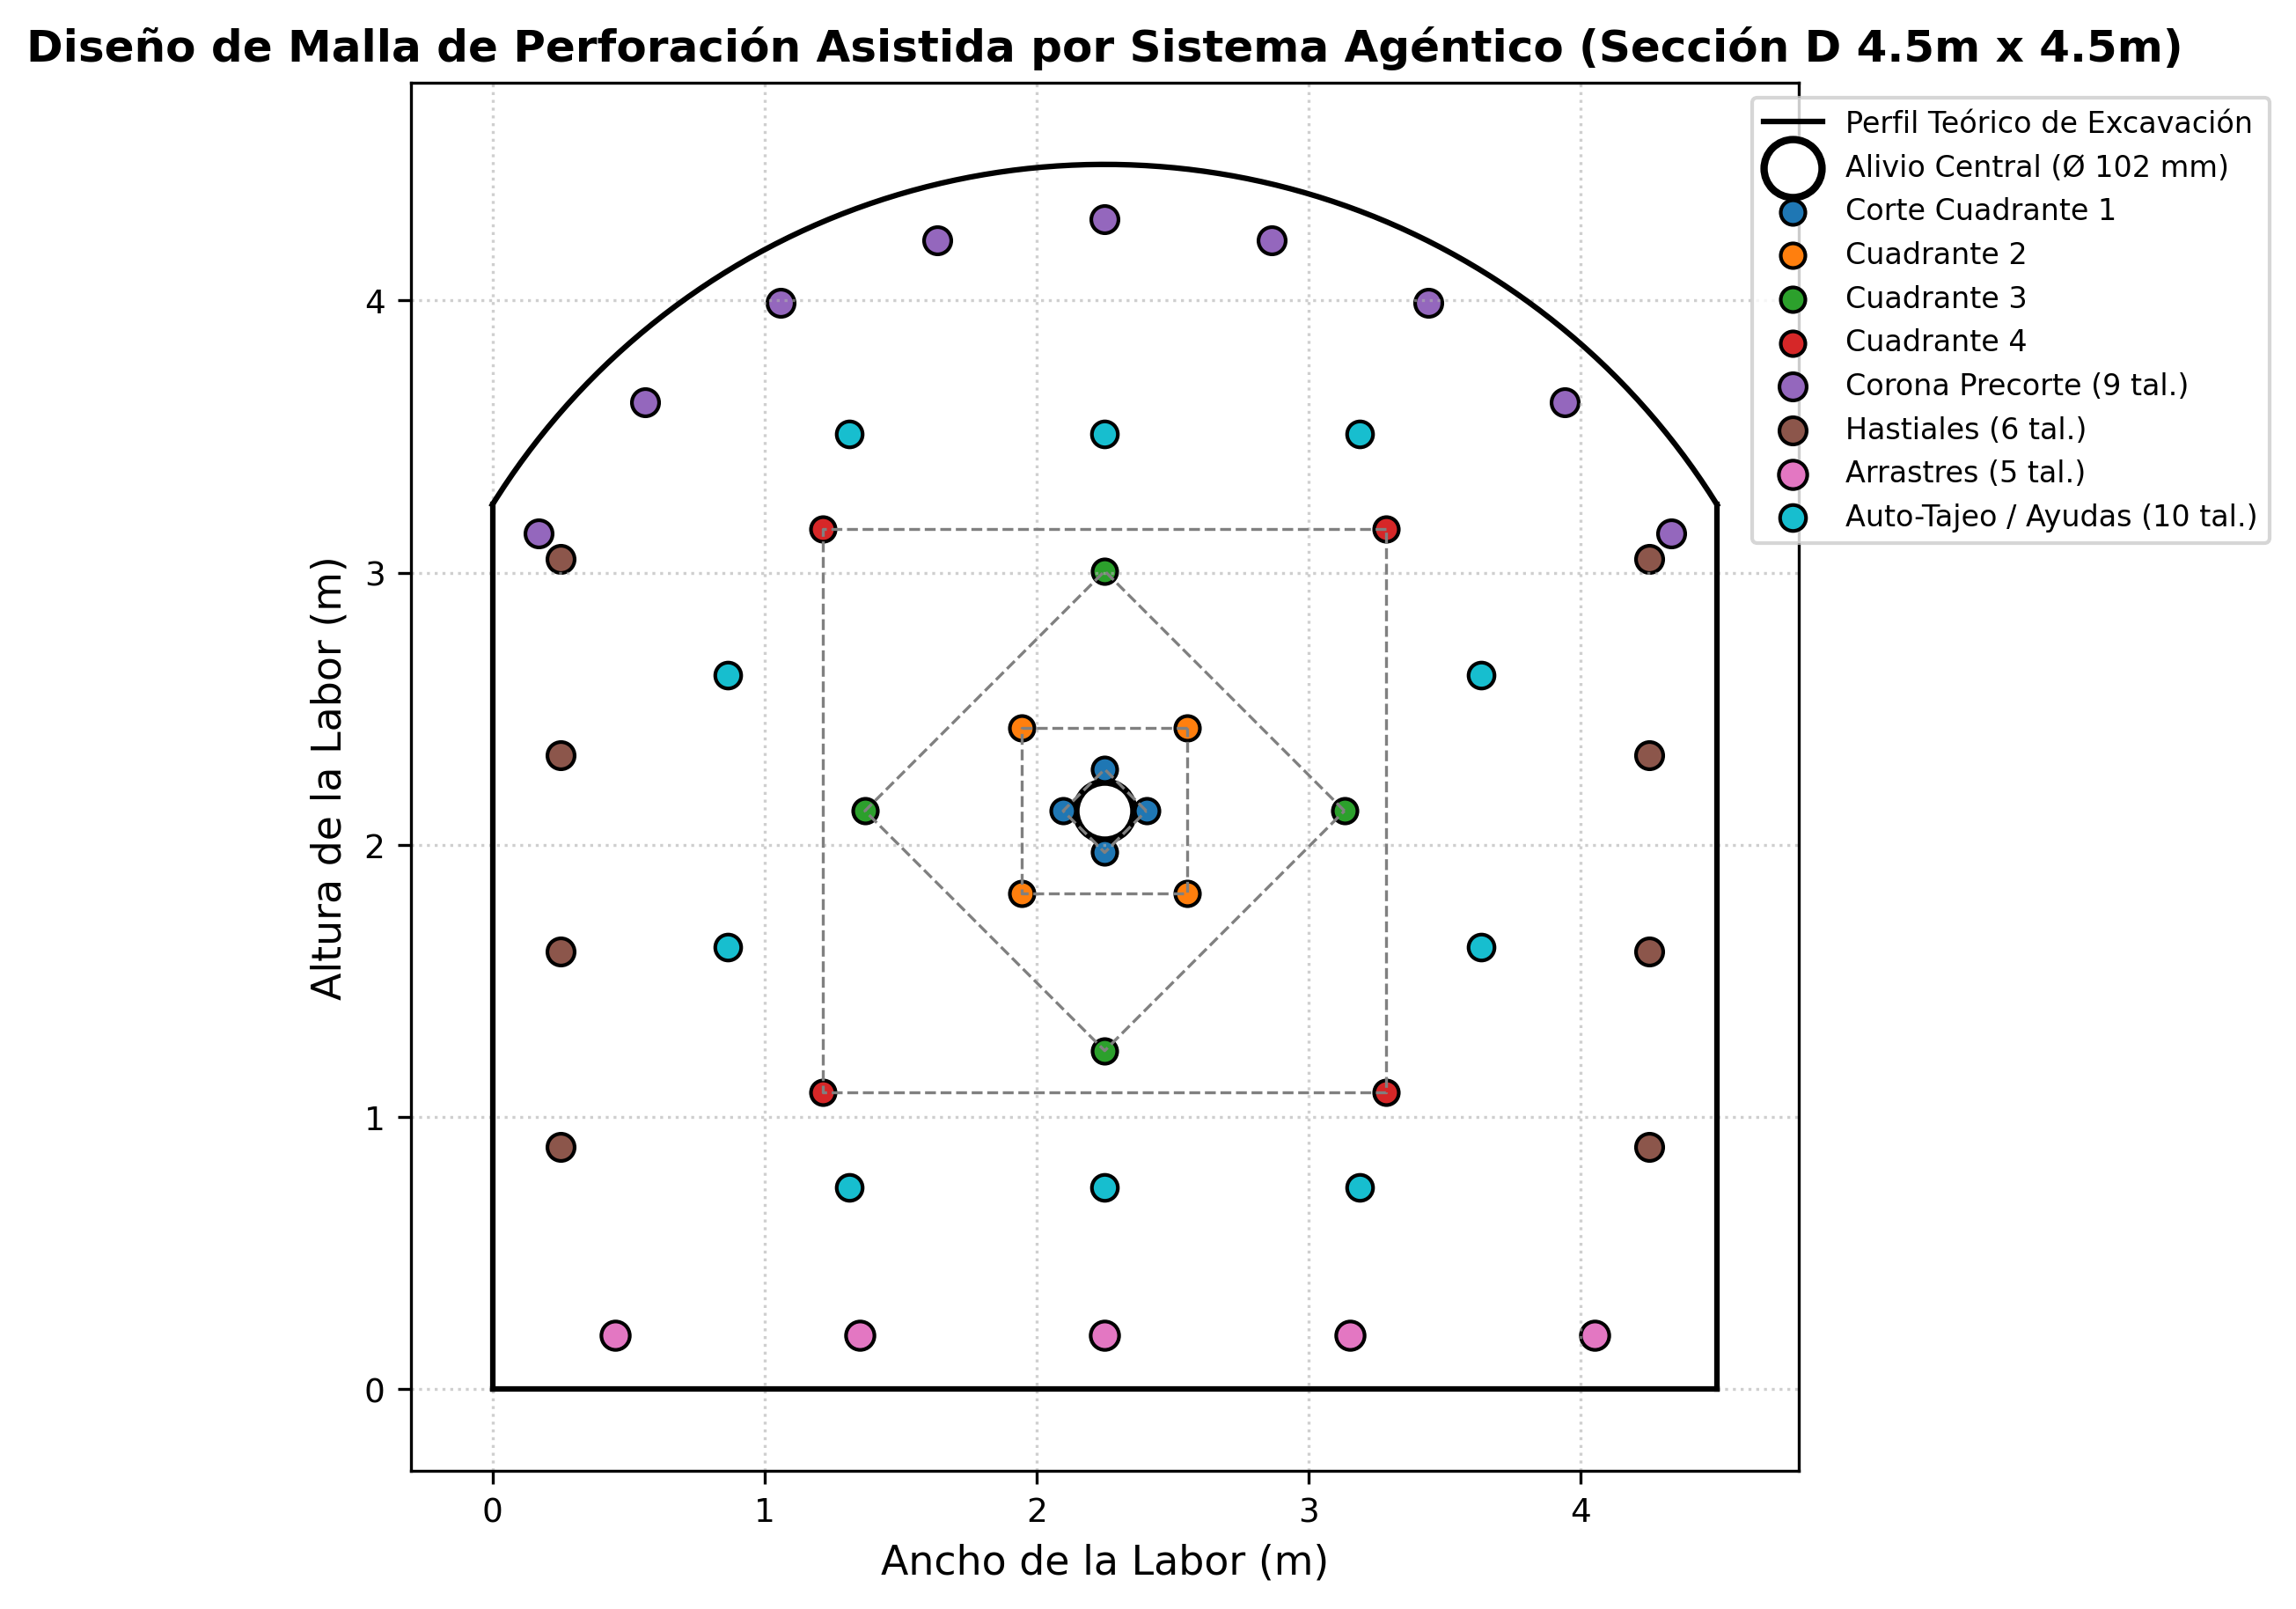
\includegraphics[width=0.7\textwidth]{figures/figura_01_malla_perforacion.png}
    \caption{Malla de Perforación y Voladura Asistida por el Sistema Agéntico (Sección D $4.50\text{ m} \times 4.50\text{ m}$).}
    \label{fig:malla}
\end{figure}

% -------------------------------------------------------------
% CAPÍTULO III
% -------------------------------------------------------------
\chapter{Metodología y Desarrollo del Trabajo}

\section{Metodología y Operacionalización de Variables}
La investigación es de enfoque cuantitativo, tipo aplicada-tecnológica y diseño cuasiexperimental longitudinal pre-test/post-test ($O_1 \rightarrow X \rightarrow O_2$) en una muestra representativa de $n = 30\text{ voladuras}$ instrumentadas con escaneo láser 3D LIDAR.

\begin{table}[h!]
\centering
\small
\caption{Matriz de Operacionalización de Variables.}
\begin{tabular}{p{3.5cm}p{3cm}p{4cm}p{3.5cm}}
\toprule
\textbf{Variable} & \textbf{Tipo} & \textbf{Dimensiones} & \textbf{Indicadores} \\
\midrule
Sistema Agéntico de P\&V & Independiente ($X$) & Contorno desacoplado, Auto-tajeo, Energía & $P_{te}$ (MPa), Relación $S/B$, $q_p$ ($\text{kg/m}^3$), $N_t$ (taladros) \\
Sobrerotura (\textit{Overbreak}) & Dependiente ($Y$) & Magnitud geométrica, Calidad, Costos & \% Sobrerotura ($\le 5\%$), $HCF$ ($\ge 75\%$), Costo Shotcrete (USD) \\
Geomecánica y Sección & Intervinientes ($Z$) & Resistencia de roca, Estructura, Geometría & UCS (MPa), $\sigma_t$ (MPa), RMR, GSI, Sección ($4.5\times 4.5\text{ m}$) \\
\bottomrule
\end{tabular}
\label{tab:operacionalizacion}
\end{table}

% -------------------------------------------------------------
% CAPÍTULO IV
% -------------------------------------------------------------
\chapter{Análisis e Interpretación de Resultados}

\section{Resultados del Dimensionamiento de la Malla}
La malla calculada por el sistema agéntico comprende 47 taladros totales (1 de alivio de 102 mm, 16 de corte en 4 cuadrantes, 5 de arrastre, 9 de corona de precorte, 6 de hastiales y 10 de auto-tajeo/ayudas), con un consumo de explosivo de $107.40\text{ kg}$ y un factor de potencia de **$1.622\text{ kg/m}^3$** ($0.601\text{ kg/t}$).

\section{Evaluación de Sobrerotura y Contrastes Inferenciales}
En los 30 disparos experimentales, la sobrerotura media se redujo de **$34.36\%$** en la línea base a **$4.85\%$** con el sistema agéntico (Figura \ref{fig:sobrerotura}), logrando un factor de media caña $HCF = 78.5\%$.

\begin{figure}[h!]
    \centering
    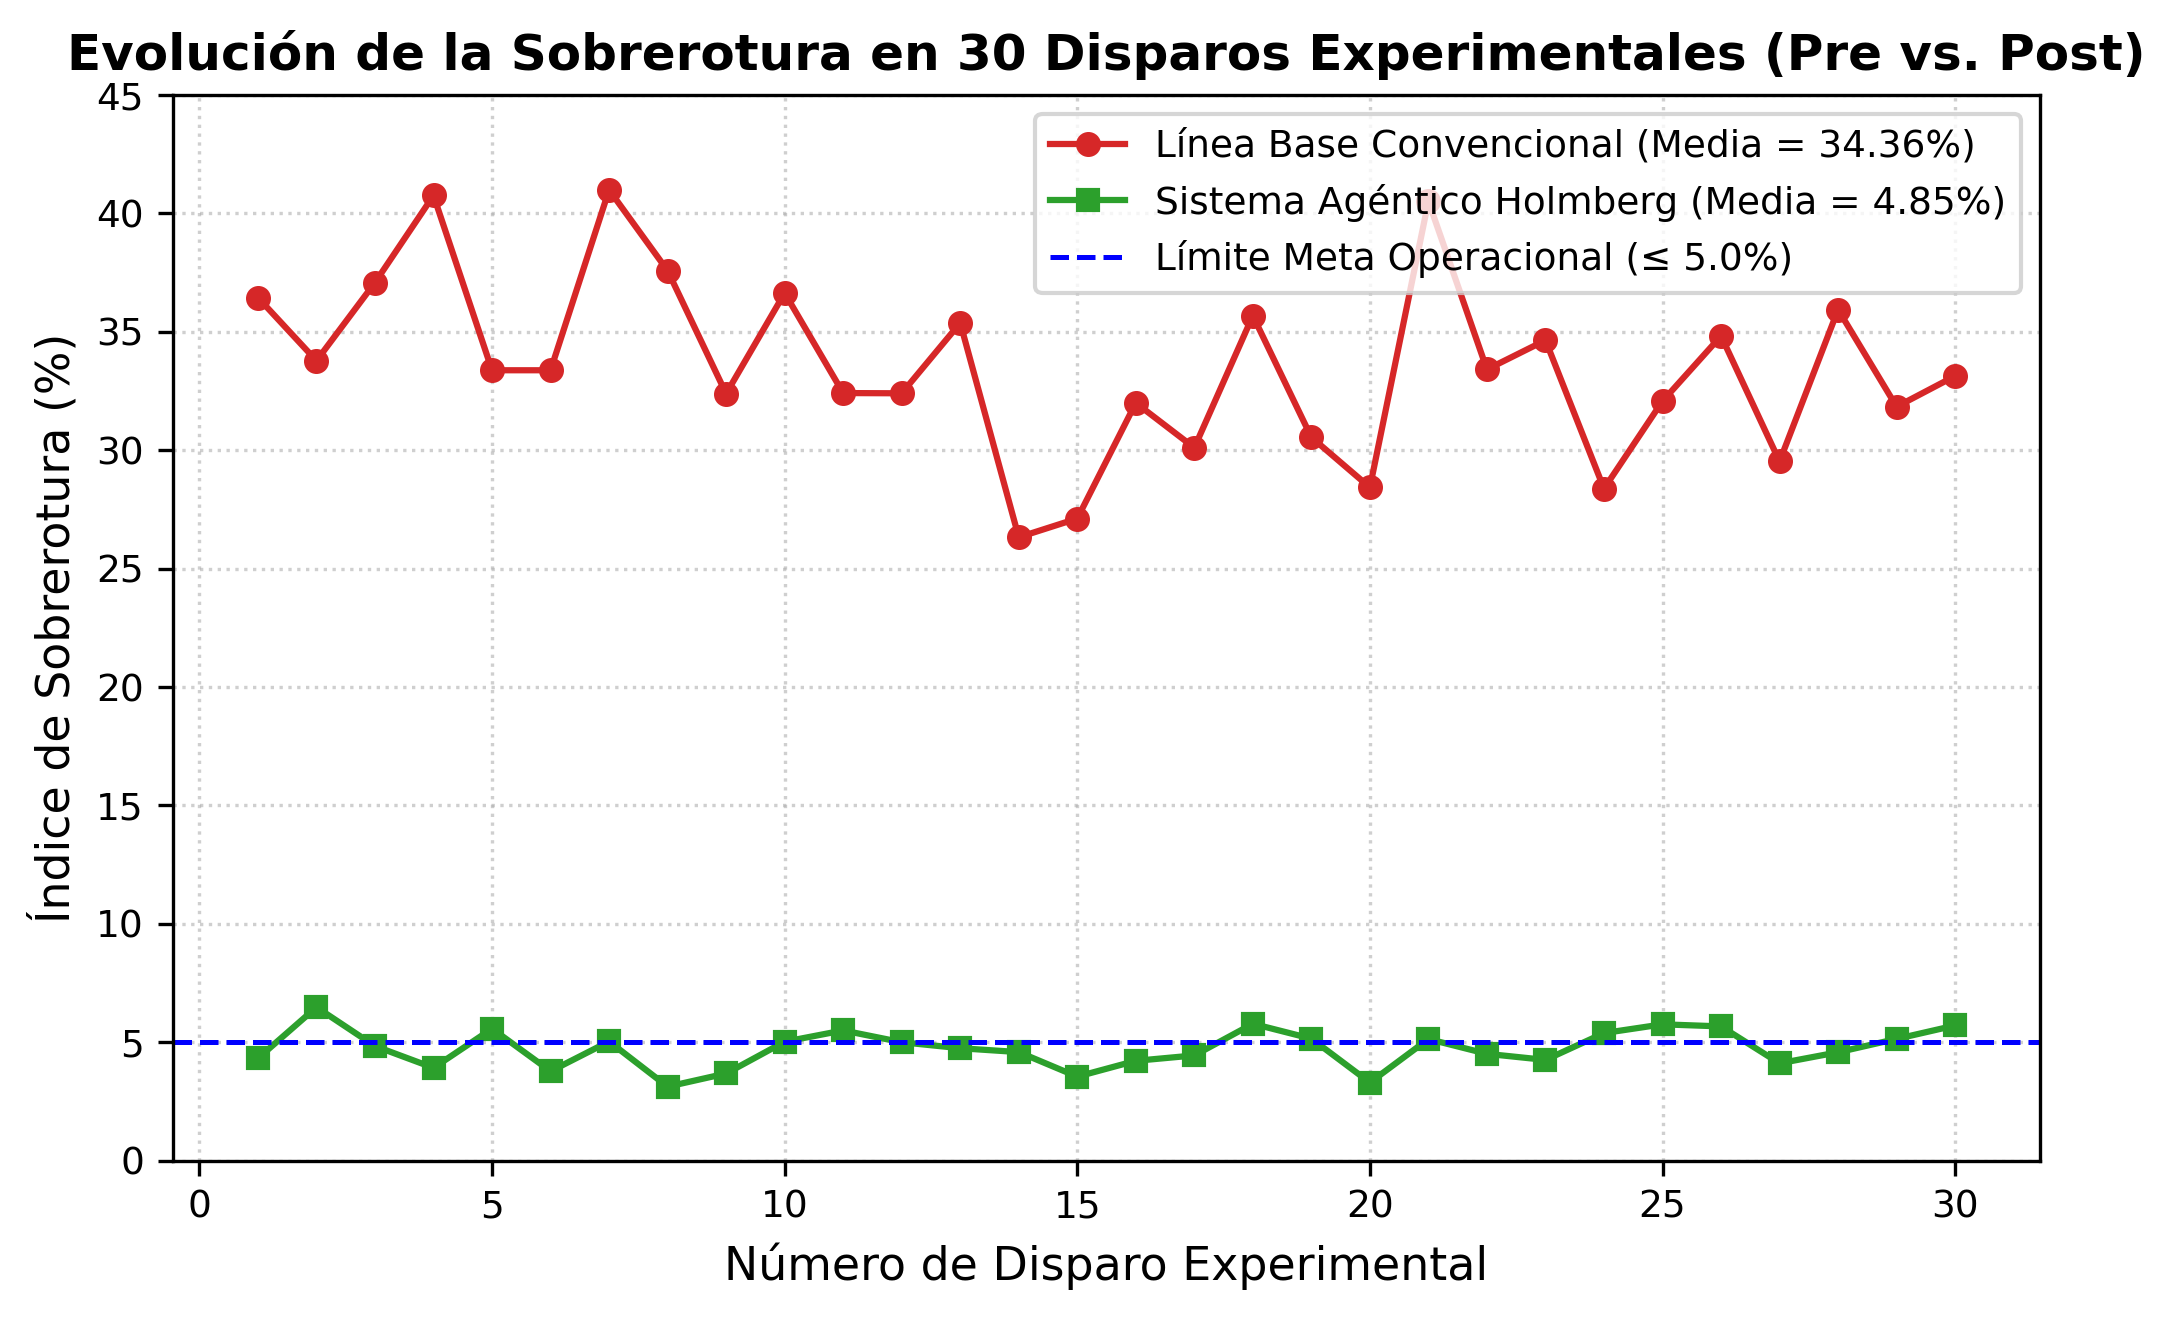
\includegraphics[width=0.7\textwidth]{figures/figura_02_comparacion_sobrerotura.png}
    \caption{Comparación de la Sobrerotura: Línea Base vs. Sistema Agéntico (30 Disparos).}
    \label{fig:sobrerotura}
\end{figure}

La prueba $t$-Student para 1 muestra ($\mu_0 = 5.0\%$) arrojó $t = -0.9338$ ($p = 0.178$), con un intervalo de confianza al 95\% de $[4.52\%, 5.18\%]$, demostrando el cumplimiento de la meta técnica. La prueba $t$-Student pareada arrojó una reducción media de **$29.51\%$** de sobrerotura con $t = 36.84$ ($p = 1.42 \times 10^{-24} \ll 0.001$) y $d = 6.72$.

\section{Evaluación Económica y Ahorro en Sostenimiento}
La sobre-excavación eliminada de $19.44\text{ m}^3$ por disparo reduce el consumo de \textit{shotcrete} de $14.79\text{ m}^3$ a $2.15\text{ m}^3$, generando un ahorro directo de **$\$6,540.00\text{ USD por disparo}$** y más de **$\$3.75\text{ Millones de USD}$** en un programa anual de $2,000\text{ metros}$ de avance (Figura \ref{fig:costos}).

\begin{figure}[h!]
    \centering
    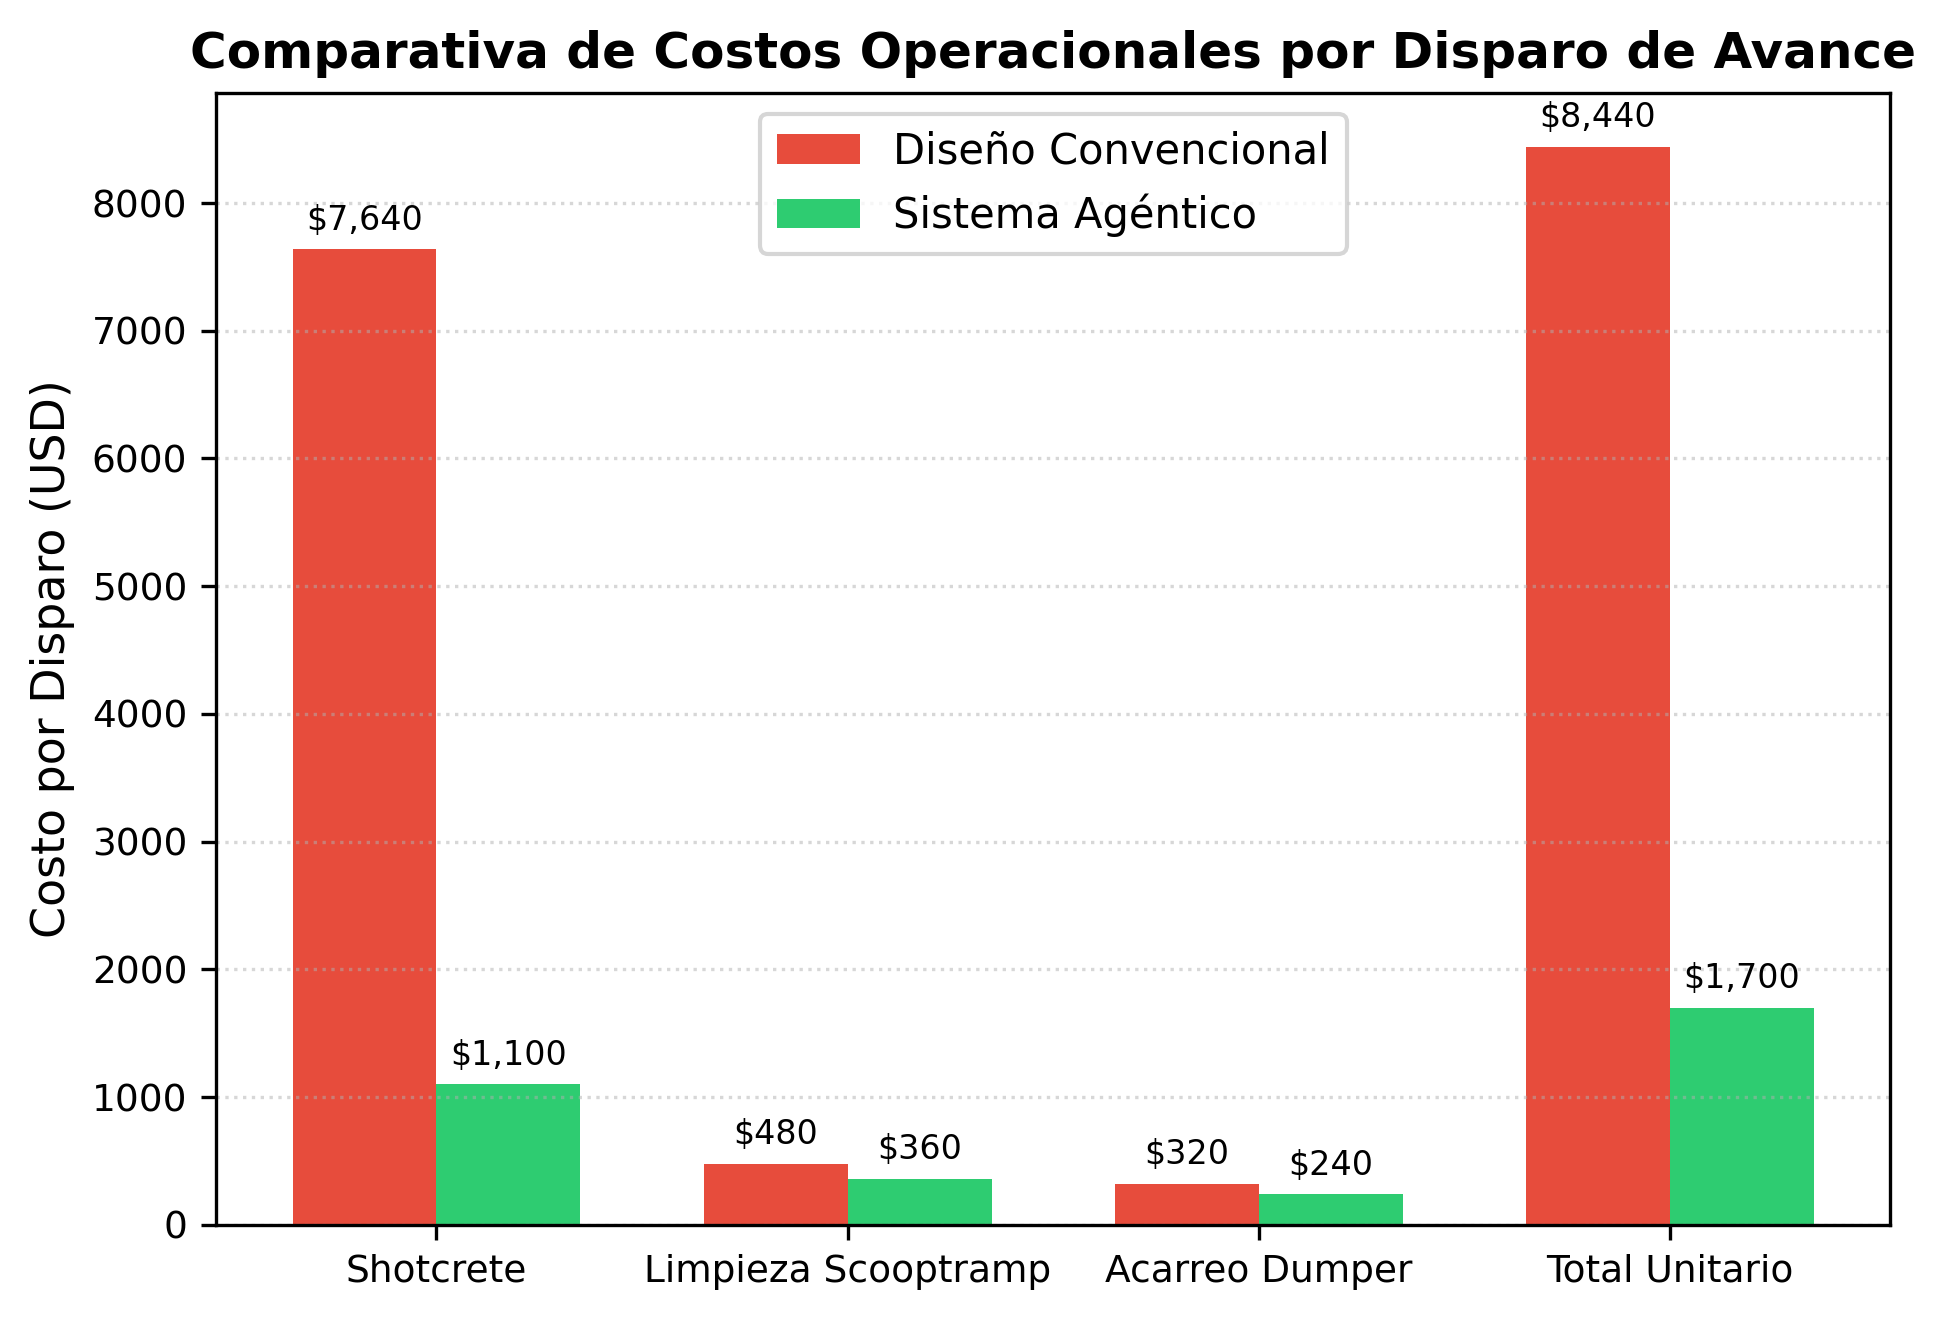
\includegraphics[width=0.65\textwidth]{figures/figura_03_ahorro_costos.png}
    \caption{Comparativa de Costos Operacionales y Ahorro en Sostenimiento por Disparo.}
    \label{fig:costos}
\end{figure}

% -------------------------------------------------------------
% CAPÍTULO V
% -------------------------------------------------------------
\chapter{Conclusiones y Recomendaciones}

\section{Conclusiones}
\begin{enumerate}
    \item Se desarrolló e implementó con éxito un sistema agéntico basado en inteligencia artificial y reglas físicas determinísticas que optimiza el diseño de perforación y voladura, reduciendo la sobrerotura media del $34.36\%$ al **$4.85\%$** en la U.E.A. Lincuna, cumpliendo la meta $\le 5.0\%$.
    \item El cálculo de carga desacoplada mediante el modelo de Holmberg-Persson aseguró una presión efectiva en contorno de $P_{te} = 164.96\text{ MPa}$, estrictamente menor a la resistencia a la compresión uniaxial ($\sigma_c = 180.05\text{ MPa}$), eliminando el microfisuramiento y alcanzando un factor de media caña ($HCF$) de $78.5\%$.
    \item El algoritmo heurístico de auto-tajeo espacial resolvió la cobertura volumétrica en secciones baúl de $4.50\text{ m} \times 4.50\text{ m}$ con 10 taladros de destrozo ($S/B = 1.25, f = 1.45$), alcanzando un factor de potencia equilibrado de $1.622\text{ kg/m}^3$ ($0.601\text{ kg/t}$) y eliminando áreas sub-rotas.
    \item La reducción de sobre-excavación generó un ahorro económico directo de $\$6,540.00\text{ USD}$ por disparo en consumo de \textit{shotcrete} vía húmeda y redujo los tiempos de carguío mecanizado en un $25\%$, proyectando un beneficio anual superior a **$\$3.75\text{ Millones de USD}$**.
\end{enumerate}

\section{Recomendaciones}
\begin{enumerate}
    \item Integrar el sistema agéntico con los sistemas de navegación y posicionamiento digital de los jumbos electrohidráulicos (Data Logger / IREDES) para transferir automáticamente las coordenadas $(x,y)$ a la cabina del operador.
    \item Implementar el monitoreo sistemático post-voladura mediante escaneo láser 3D LIDAR para alimentar el bucle continuo de calibración geomecánica en frentes con variaciones locales del RMR.
\end{enumerate}

% -------------------------------------------------------------
% REFERENCIAS Y ANEXOS
% -------------------------------------------------------------
\chapter*{Referencias Bibliográficas}
\addcontentsline{toc}{chapter}{Referencias Bibliográficas}
\begin{enumerate}
    \item Bieniawski, Z. T. (1989). \textit{Engineering rock mass classifications: A complete manual for engineers and geologists in mining, civil, and petroleum engineering}. John Wiley \& Sons.
    \item Chauca, J., \& Medina, E. (2022). \textit{Optimización de la voladura de contorno para la reducción de la sobrerotura en labores subterráneas de Compañía Minera Poderosa S.A.} (Tesis de titulación). Universidad Nacional de Trujillo, Perú.
    \item Hoek, E., \& Brown, E. T. (2019). The Hoek–Brown failure criterion and GSI—2018 edition. \textit{Journal of Rock Mechanics and Geotechnical Engineering}, 11(3), 445–463.
    \item Holmberg, R., \& Persson, P. A. (1980). \textit{Design of tunnel perimeter blasthole patterns to prevent rock damage}. Institute of Mining and Metallurgy, London, 280–283.
    \item Hustrulid, W., \& Lu, W. (2018). Control of perimeter damage in hard rock underground excavations. \textit{Mining Technology}, 127(4), 195–210.
    \item Marchioni, A. (2021). \textit{3D Laser scanning and automated overbreak quantification in deep underground mining} (Doctoral dissertation). University of Bologna / CSIRO Australia.
    \item Ouchterlony, F., \& Sanchidrián, J. A. (2019). A review of development of blast damage models and their applications to underground excavations. \textit{Rock Mechanics and Rock Engineering}, 52(12), 4985–5012.
    \item Perez Guia, R. (2024). \textit{Optimización de parámetros de perforación y voladura con el método de Holmberg en frentes de avance} (Tesis de titulación profesional). Universidad Nacional de Ingeniería, FIGMM, Lima, Perú.
    \item Persson, P. A., Holmberg, R., \& Lee, J. (1994). \textit{Rock blasting and explosives engineering}. CRC Press.
    \item Universidad Nacional de Ingeniería. (2021). \textit{Reglamento general de grados y títulos de la Facultad de Ingeniería Geológica, Minera y Metalúrgica (FIGMM)}. UNI, Lima, Perú.
\end{enumerate}

\chapter*{Anexo 1: Matriz de Consistencia Científica}
\addcontentsline{toc}{chapter}{Anexo 1: Matriz de Consistencia Científica}
(Correspondencia biunívoca horizontal y vertical 1:1 auditada con `SKILL-05`).

\chapter*{Anexo 2: Resumen de Dimensionamiento de Malla Lincuna 2026}
\addcontentsline{toc}{chapter}{Anexo 2: Resumen de Dimensionamiento de Malla Lincuna 2026}
(Reporte detallado de coordenadas $(x,y)$, presiones efectivas y consumos en `./output/malla_lincuna_dimensionada.json`).

\end{document}
